\section{Technical Testing}\label{sec:technical}


\replace{V}{As explained above, v}erification \replace{is to check}{means checking} whether the software conforms to specifications. This type of evaluation and testing will be primarily reported and covered in the \ins{deliverables of the} different technical work packages. However, a brief overview of the main evaluation techniques planned for the different technologies is provided below.

\subsection{Verification Phases}\label{sec:verification}

The \textbf{user requirements} outlined in D1.1 Use Case Descriptions and Requirements, describing user requirements, user expectations and personae, serve as starting point for the \SUMMA platform development and design.

\textbf{Functional specifications} for each of the components, as well as the integrated platform, are derived from the user requirements. The functionality of each component is tested and reported in the respective work packages WP3-5.

Testing of the \textbf{integrated platform} is done primarily by \SUMMA integrator LETA throughout the project duration and reported in WP6.

User Interfacing and \textbf{demonstrator design} on top of the integrated platform is developed in close collaboration with the user partners and tested against user specifications. 

Two major levels for technical evaluation, i.e., component-level testing and integrated platform testing, are described in more detail below.

\subsection{Component Testing}\label{sec:component}

The following technologies/components are covered:
\begin{itemize}
\item ASR: Speech recognition
\item Meta: Metadata extraction from broadcast media
\item MT: Machine translation
\item CT: Streaming implementation of Storyline Clustering and Topic detection 
\item ETL: Entity Tagging \& Linking 
\item KB: Knowledge Base Construction
\item FC: Forecasting and Fact Checking
\item SP: Story-level semantic parsing 
\item SH: Story highlight generation/summarisation
\item SS: Story-level sentiment analysis
\end{itemize}

Key performance indicators that we will measure against will include Test Value, Sample Average, Sample Size, Standard Deviation for Sample, Confidence Interval, and Statistical Power\ins{, where applicable}.
%\UG{I don't think anyone ever computes Statistical Power for MT evaluation.}

Additionally, we will perform \SUMMA platform scalability tests prior to project months M24 and M36 to verify key performance indicators:
\begin{itemize}
\item sub-minute latency for shallow stream processing (including speech recognition, machine translation, and metadata extraction)
\item 10,000 tokens per second for semantic analytics (entity linking and natural language understanding tasks)
\end{itemize}

Although the platform architecture will be highly parallelised and cloud-scalable to large number of input streams, some functional modules such as clustering into story-lines need to cut across all input streams simultaneously. We envision the final scalability test to be run on 250–400 parallel news streams (in the external \ins{use} case).

The scalability tests will require computing clusters of significant size\replace{ – i}{. I}f internal resources will not be sufficient, we will
temporarily \replace{employ}{use} Amazon EC2 and EC3 \ins{cloud computing} services during scalability tests.

KPIs that are specific to the internal monitoring use case include the volume of material that has been monitored by other language departments and the percentage of reused material (rather than the volume, as this depends on high or low news traffic of the day or week.) 

The external use case protocol will evaluate data streams and the semantic level.


\subsubsection{Automatic Speech Recognition (ASR)}

Models for ASR are universally evaluated using word error rate (WER); this metric incorporates substitutions, insertions and deletions of words compared to a human generated transcription.

In the context of \textbf{model development}, we will evaluate models on fixed test sets that are typically provided with training data corpora. Such test sets are available for most of the better resourced languages developed for the \SUMMA platform.  Use of these test sets has the advantage \replace{of being}{that these are} standardised within the community, so that performance can be compared across labs without sharing implementations.  To ensure that our systems are competitive with the state-of-the-art, we will also participate in the MGB Challenge, an open competition evaluating ASR system on English and Arabic TV broadcasts. 

In the context of \textbf{unit tests} in the \SUMMA platform, we will \replace{further}{additionally} evaluate models on manually transcribed test data provided by the project.  Such results are likely to be slightly worse than those of the conditions above.  This is partly because the project test data will be mismatched to the training corpora in terms of speakers and recording conditions, and partly because we expect project data to be fundamentally more challenging for ASR due to the possible presence of background noise and music.

We will \replace{distinguish}{consider} real-time and off-line systems.  \replace{In the lab}{Under laboratory conditions}, state-of-the-art results are likely to come from off-line systems, owing to their using multiple passes, as well as models such as the  BLSTM (Bidirectional Long Short-Term Memory), which operate on long chunks of speech; \ins{however,} these methods cannot be made to operate in a real-time manner.  Real-time systems\cut{, however,} aim to run at least as fast as real speech and produce output as soon as possible after each word has been spoken.  Generally, we would expect real-time systems to be slightly worse in terms of WER.

The real-time requirement \replace{leads to a requirement to}{forces use to also} consider ASR decoding speed.  The most important factor affecting this is the ``beam width'' used in the search for the best output for each utterance.  For each model that is developed for the \SUMMA platform, we will evaluate its WER when the beam width is set to a value that results in a real-time decoding speed on given hardware, when averaged over the whole test set. 

It may also be appropriate to evaluate ASR WER after correction by a downstream MT system. However, in the context of this document, the case is equivalent to the offline system described above.

\subsubsection{Metadata extraction from broadcast media (Meta)}

The metadata extraction module will be used to obtain speaker and punctuation information from broadcast data.  The 
speaker and punctuation extraction will be evaluated separately.  

Punctuation will be evaluated with respect to human-generated captions for the \SUMMA test data.  When the punctuation is inserted into ASR output, this will be automatically aligned to the human captions to match up the candidate punctuation slots between words.  
We will use an F-measure to evaluate punctuation prediction accuracy across all punctuation marks: full stop, comma, question mark, etc; we will also obtain a general slot F-measure, conflating all punctuation marks.

Speaker diarization and linking performance will be evaluated with respect to the standard Diarization Error Rate (DER) metric defined by NIST.  To ensure comparability with the other systems, we will evaluate DER on the speaker diarization track of the English MGB Challenge, as well as on multilingual test sets defined by the project.  We will also evaluate speaker change detection using the F-measure, where each adjacent pair of spoken utterances is considered as a potential speaker change point.


\subsubsection{Machine Translation (MT)}

\cut{%
The MT modules that we develop for \SUMMA will be evaluated at every stage of their development.}  

\replace{%
We will evaluate the quality of our models by applying%
}{% WITH
MT performance will be evaluated continuously in terms of
} % END OF REPLACEMENT
commonly used automatic metrics, such as BLEU and CHRF1, 2 and 3  METEOR and TERp. This will mean we can report using metrics which are well understood by the MT community and capture different aspects of translation performance. 

In order to establish the quality of our systems with comparable baselines, we will compete in open shared tasks. We will compete in the \ins{Shared Task on News Translation at the annual} \textit{Conference on Machine Translation} (WMT)\cut{\ shared task which has a news track}, and the \textit{IWSLT} shared task, which has a spoken language translation task. \cut{Both of these tasks are very relevant to \SUMMA.} This will allow us to know how we compare to the world's best research labs and to the most widely used commercial translation systems. 

Automatic metrics need human translated test sets to benchmark the system performance. \replace{The}{Test sets for} \SUMMA \cut{test sets} are currently being created, and as soon as they are available, each iteration of the \SUMMA MT tools will be evaluated according to these test sets\replace{. Hopefully this can be done automatically with a regression test in the \SUMMA platform}{\ as part of the automated MT testing pipeline}. Until the \SUMMA test set is available, we will use the latest WMT and IWSLT test sets\replace{ as our gold standard test data}{instead}. 

% added by APB:
\replace{Particularly, t}{T}he coreference-aware MT component will be tested in terms of the accuracy of noun phrase and$\,$/$_{\,}$or pronoun translation, using dedicated metrics such as APT (Accuracy of Pronoun Translation, developed at IDIAP).  APT scores the number of identical, different, or missing pronouns, using alignment.  For research on this MT component, a controlled Spanish-English News Commentary subset \ins{from WMT} is used \cut{(from WMT)}, \replace{as}{since} gold co-reference resolution is available \replace{on}{for} it, and \ins{since} manual evaluation is possible thanks to its limited size.  However, any parallel test set can be used with the APT metric if it has a reference translation.  An extension of APT to nouns is under study, and will be compared to reference-based metrics such as METEOR which can also be restricted to specific parts-of-speech such as nouns, or, alternatively, to named entities.

\replace{We will also need to benchmark our translation models in terms of their}{Our MT engines will also be benchmarked with respect to translation} speed. We will measure the number of words and sentences translated per second, and compare this to a number of other popular MT decoders. Trade-offs between model quality and speed will be measured to determine good settings for \replace{beam size and the number of models in ensembles}{parameters that affect speed and translation quality}. \cut{Model training times will be reported, but this measure is less critical to the success of the \SUMMA project.}

Because translation is not performed in isolation to the other \SUMMA components, we will also provide evaluations of MT performance in the \SUMMA pipeline. We will measure the speed and quality of translation with broadcast media passed through the full pipeline of speech recognition, segmentation and punctuation, and machine translation. 


\subsubsection{Clustering and Topic Labelling (CT)}

Automatic measures will be used to assess research and development efforts of the Clustering technology using the standard metrics Precision (P), Recall (R), F1, Purity, Rand Index (RI) and Adjusted Rand Index (ARI) against development clustering datasets from the literature. To this end, we have been using the multilingual clustering dataset from the work in \citet{Rupnik16News}\cut{, internally called the JAIR dataset}. Since it is difficult to find such datasets with fine clusters, and evaluation is always biased to what the authors considered a cluster, user evaluation and feedback is specially important for the clustering component.

The clustering technology will also be evaluated \replace{regarding}{with respect to} computing speed. The input to this module will be news documents and ASR/MT data streams already segmented as stories (documents) from previous modules, which may total the predicted 250-400 parallel \SUMMA streams. As such, performance will be measured in terms of clustered documents per second. The resulting performance will be deemed acceptable if the module can cope with the required data streams.

According to the current problem setting, an incoming document either creates a new cluster or joins an existing one, therefore influencing all subsequent clustering choices. In a first instance, we'll keep this setting and approach the problem using a single software module to cluster all data streams and benchmark it to assess performance. According to this assessment, we may decide that optimising a centralised module is enough or that we need to change the problem setting to allow the system to scale. In the latter case, a relaxation of the setting may be devised, such as computing clusters in parallel and merge them across streams (or groups of streams) to obtain the final clusters.

As for topic labelling or detection, this is evaluated using mainly the F1 score, i.e.\ the average of precision and recall.  This is computed separately for each label appearing in the data.  For a given label, precision and recall are computed for the retrieval of the documents with that specific label in the reference data.  Then, the F1 scores for all the labels are averaged to produce a unique score for the task.  Typically, we use micro-averaging so that the scores per labels are weighted, in the average, by the frequency of the label.

This automatic metric requires the availability of labelled data: in our experiments, we take advantage of the Deutsche Welle collection, gathered by Priberam, with documents in 8 languages (all \SUMMA languages except Latvian) with two types of topic labels (or keywords): coarse-grained vs.\ fine-grained. Each language contains between 35k and 130k documents, with 28--367 different coarse-grained topic labels (categories) and 127--1058 fine-grained labels (keywords).  We also consider a multilingual dataset of TED transcripts.  The main goal is to demonstrate that neural networks with an attention mechanism can learn multilingual representation that enable transfer from high to low-resource languages.


\subsubsection{Entity Tagging \& Linking (ETL)}

\ins{The} Entity Tagging and Linking (ETL) module will be evaluated, at every stage of its development, as a standalone task. For that purpose, we will use well-established datasets, such as the ones distributed for the TAC-KBP shared tasks and the AIDA-CONLL corpus. \citep{Hoffart11Robust} The system performance will be measured with the standard metrics that are used for evaluating those datasets. \replace{In particular, that automatic evaluation includes computing different scores that account for the various dimensions of the module, namely for}{These include}: (1) the correct identification of mentions in text; (2) the correct classification of mentions with entity types (such as PER, GPE, ORG, etc); (3) the correct classification of mentions with entities in a knowledge base (4) and the correct cross-document clustering of coreferent mentions whose entities may not yet be in the knowledge base.

The ETL system will be compared against state-of-art technologies by evaluating on standard metrics and datasets and by competing in the Text Analysis Conference -- Knowledge Base Population (TAC-KBP) shared tasks. These tasks are very aligned with \SUMMA goals both in terms of the tasks and of the languages that are covered. We have already participated in the TAC-KBP 2015 where we have scored as an intermediate system at the task of Entity Discovery and Linking (EDL) \citep{Paikens16SUMMA}. From this competition we concluded that, at that stage, the bottleneck of the ETL module was the mentions detection system, while the step of linking the mentions to knowledge base entries was on pair with the top competing systems.

We will also \cut{need to} benchmark the ETL models in terms of their speed. We will measure the number of words, sentences and mentions processed per second, and compare these numbers with those of other state-of-art systems. We will report \ins{numbers for} different models with different qualities and speeds.

\subsubsection{Knowledge Base Construction (KB)}

Our current evaluation is based on the shared TAC-KBP task, using standard metrics such as accuracy, precision, recall and F1.

As \SUMMA data becomes available, \replace{it would be ideal to then}{we plan to} evaluate \ins{knowledge base construction} within the full pipeline. This \replace{would}{will} allow us to understand the challenges introduced by working with the outputs of ASR and MT.
\replace{However, this requires a \SUMMA test set.
We currently have a sample of the BBC Monitoring Research knowledge base and are investigating the feasibility of employing this for evaluation purposes.}{We are currently investigating whether an existing sample of the BBC Monitoring Research Knowledge Base is suitable for evaluation purposes until a \SUMMA test set is available.}

\subsubsection{Fact Checking (FC)}

A first evaluation will use knowledge base population as a proxy task: if we can recognise claims in text correctly, then we can populate the knowledge base. Thus we will follow the TAC-KBP task, using standard metrics such as accuracy, precision, recall and F1. In this regard, we will also investigate how we can use the BBC monitoring data for the evaluation.
To evaluate the fact-checking capabilities more directly we will also work on evaluating the system developed using the data provided for an upcoming competition\cut{ announced here:}%
\footnote{\url{http://www.fakenewschallenge.org/}}\cut{ by researchers in machine learning}. The domain is news and and the goal is to assess headlines as true/false and provide provenance. The evaluation metric used will be accuracy, i.e. how many truth assessments were found to be correct.

\subsubsection{Story-level semantic parsing (SP)}

The parser that \replace{has been developed}{we have developed for \SUMMA} is an abstract meaning representation (AMR) parser, with a first version for English and subsequent versions for German and Spanish. For English, we use a standard evaluation dataset for AMR, together with a standard evaluation metric called SMATCH. SMATCH measures the similarity of two graphs (one being the output of the parser, an AMR graph, and the other being the gold-standard AMR graph) by trying to build an alignment as close as possible to an isomorphism between the two graphs. 
AMR datasets mostly exist for English, and as such, we would devise different techniques to automatically evaluate the German and the Spanish parsers.
We believe that by the end of February we will have an automatic evaluation of the parser for German and Spanish. \cut{There was already a paper published about evaluating our parser for English (Damonte et al., EACL, 2017)}\ins{Evaluation results using this the standard procedure for our English AMR parser are provided in \citet{damonte-17}.}

\replace{In addition, w}{W}e are \ins{also} planning to participate in the SemEval \ins{Shared T}\cut{t}ask this year\cut{ and have our AMR parser compete with others} (English only).
We have also found some weaknesses in the current evaluation techniques with the SMATCH score. As such, in a recent EACL paper \citep{damonte-17}, we introduced a suite of evaluation metrics for AMR which we will use to test our parsers. The set of metrics is also available for review \replace{here:}{at}
\url{http://kinloch.inf.ed.ac.uk/amr-evaluation.html}

\subsubsection{Story Highlight Generation and Summarisation (SH)}

The standard metric to evaluate summarisation is ROUGE \citep{Lin04ROUGE}, a n-gram overlap of the predicted summary among the model human summaries.

Other common metrics such as Linguistic Assessment and Pyramid \citep{Nenkova07Pyramid} are not going to be adopted since they require manual efforts. The assessment of the quality of the summary is understood to happen in the software validation step.

For conducting the evaluation we will consider the datasets provided by the main shared tasks on summarisation (TAC and DUC) as well as new datasets that explore the concept of highlights summary such as the CNN/DailyMail dataset \citep{ChengLapata16Neural}.

The former has the advantage of exploring multi-document clusters and also, they are well recognised and easy to compare with state-of-art approaches. The later focuses only on single document summarisation. However, it aims to generate summaries in terms of highlights which is closer to our project needs, in comparison to the former where summaries are presented as long text. 

In addition, a third dataset may be annotated in the context of \SUMMA project. This would offer the benefits of multi-document input (closer to what we consider a story-line) and the output in highlights, thus taking the full advantage of our summarisation approach.

The system reported will be scored against standard baselines such as frequency-methods, basic entity-graph methods and coverage-based summarisation models.


\subsubsection{Story-Level Sentiment Analysis (SS)}

The evaluation of sentiment analysis component will use standard text classification measures such as Precision, Recall and F-Measure. 

The evaluation will be conducted in SemEval datasets for Sentiment Analysis in Tweets \citep{Nakov13SemEval, Rosenthal14SemEval, Rosenthal15SemEval, Nakov16SemEval}


\subsubsection{Schedule of Component Release}

The anticipated release dates of specific technical components are listed below. The availability of these components determines the timing of the planned (user) evaluation.
%\UG{Remove the ``Component Component Component ...'' column in Fig.~3. Also, the image is too wide. - done}

%\begin{figure}[ht]
%    \centering
%    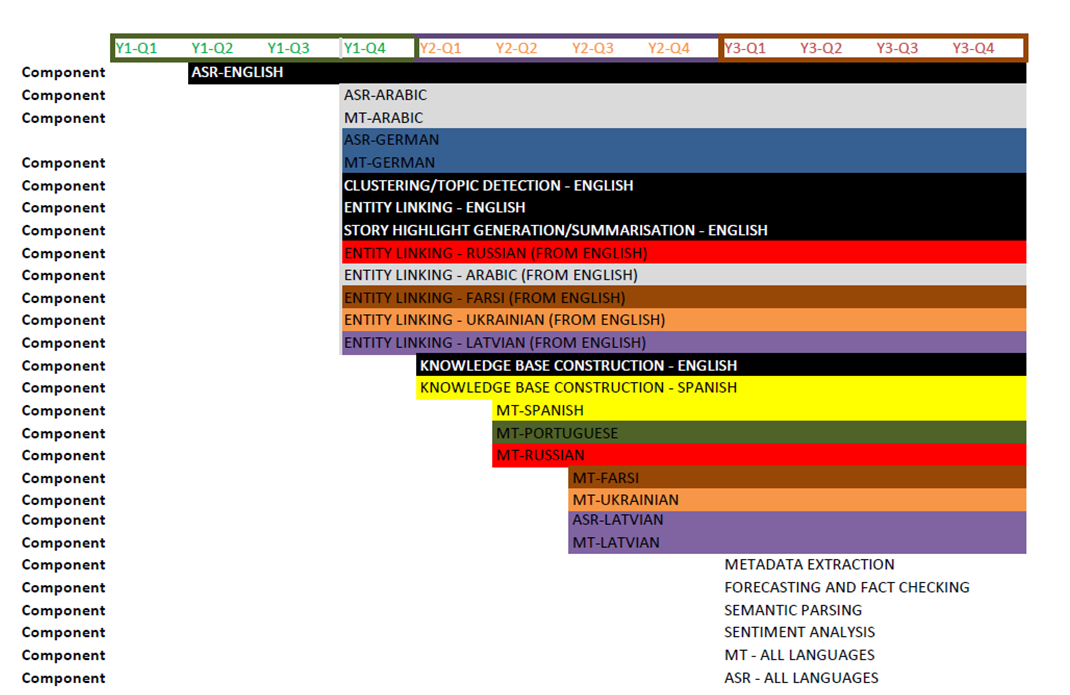
\includegraphics[width=1.1\textwidth]{./images/evaluation_time_schedule_v3_3.png}
%    \caption{Anticipated Schedule of Component Release}
%    \label{fig:Evaluation Planning Time Schedule}
%\end{figure}



\begin{figure}[ht]
    \centering
    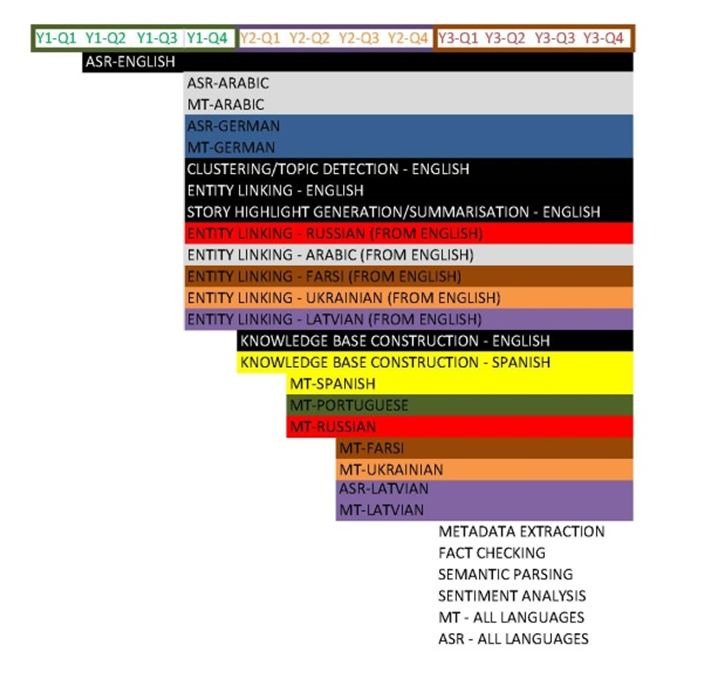
\includegraphics[width=1.0\textwidth]{./images/evaluation_timing_v5.png}
    \caption{Anticipated Schedule of Component Release}
    \label{fig:Evaluation Planning Time Schedule}
\end{figure}







\begin{comment}

Probably add a user trial in Y2-Q2. 
Is the generic prototype sufficient for such a user trial, or do we need to push dashboarding forward, into Y2-Q2?

Based on the information available after the Lisbon meeting. This image will be updated when more info becomes available

Need timing for: 
LETA prototype
Internal monitoring
External monitoring
ASR per language
MT per language
Clustering (as of Dec 2016)
Summarization 
\end{comment}

\subsection{Integrated Platform Testing}\label{sec:IP}

Additionally, we will perform \SUMMA platform scalability tests prior to project months M24 and M36 to verify key performance indicators:
\begin{itemize}
\item sub-minute latency for shallow stream processing (including speech recognition, machine translation, and metadata extraction)
\item 10,000 tokens per second for semantic analytics (entity linking and natural language understanding tasks)
\end{itemize}

Although the platform architecture will be highly parallelised and cloud-scalable to large number of input streams, some functional modules such as clustering into story-lines need to cut across all input streams simultaneously. We envision the final scalability test to be run on 250–400 parallel news streams (in the external \ins{use} case).

The integration platform is highly modular due to Docker containerisation of all components via Docker Compose interconnect mechanism. Thus, the only top-level component of the integrated system is merely a docker-compose.yml configuration file, which defines how the individual Docker containers are started and how they are interconnected to emerge the entire \SUMMA platform.

This architecture guides the evaluation process of the integrated platform --- unit-testing of individual Docker containers and overall testing via Docker Compose. The integrated system shall be self-reporting in the sense that each module should detect abnormal inputs or behaviours and report them using the appropriate logging facility along with the brief logging of the normal processing of data to provide the context to their modules, where the problem occurs. In this respect, the \SUMMA integration platform debugging and technical evaluation is similar to the networked system debugging, where event logging is the primary source of debugging information.

For integration testing, the platform can work on a predefined testing dataset. The platform saves the output and processing time of every test document for each NLP module. After every major update to some of the NLP modules, the whole system is run on the testing dataset. If an NLP module produces an error on a test document, the corresponding call and data will be sent to the module's author for investigation. A similar procedure will be followed if there is a regression in processing time. 

The scalability tests will require computing clusters of significant size\replace{ – i}{. I}f internal resources will not be sufficient, we will
temporarily \replace{employ}{use} Amazon EC2 and EC3 \ins{cloud computing} services during scalability tests.

KPIs that are specific to the internal monitoring use case include the volume of material that has been monitored by other language departments and the percentage of reused material (rather than the volume, as this depends on high or low news traffic of the day or week.) 

The external use case protocol will evaluate data streams and the semantic level.

Integrated Platform testing will be reported in detail in WP6. 